\documentclass[../rapport.tex]{subfiles}
\graphicspath{{\subfix{ressources/photos_diagrammes/app1/}}}

\usepackage[utf8]{inputenc}
\usepackage[french]{babel}
\usepackage{amsmath, amsfonts, amssymb, amsthm}

\begin{document}

\begin{figure}[h!]
		\centering 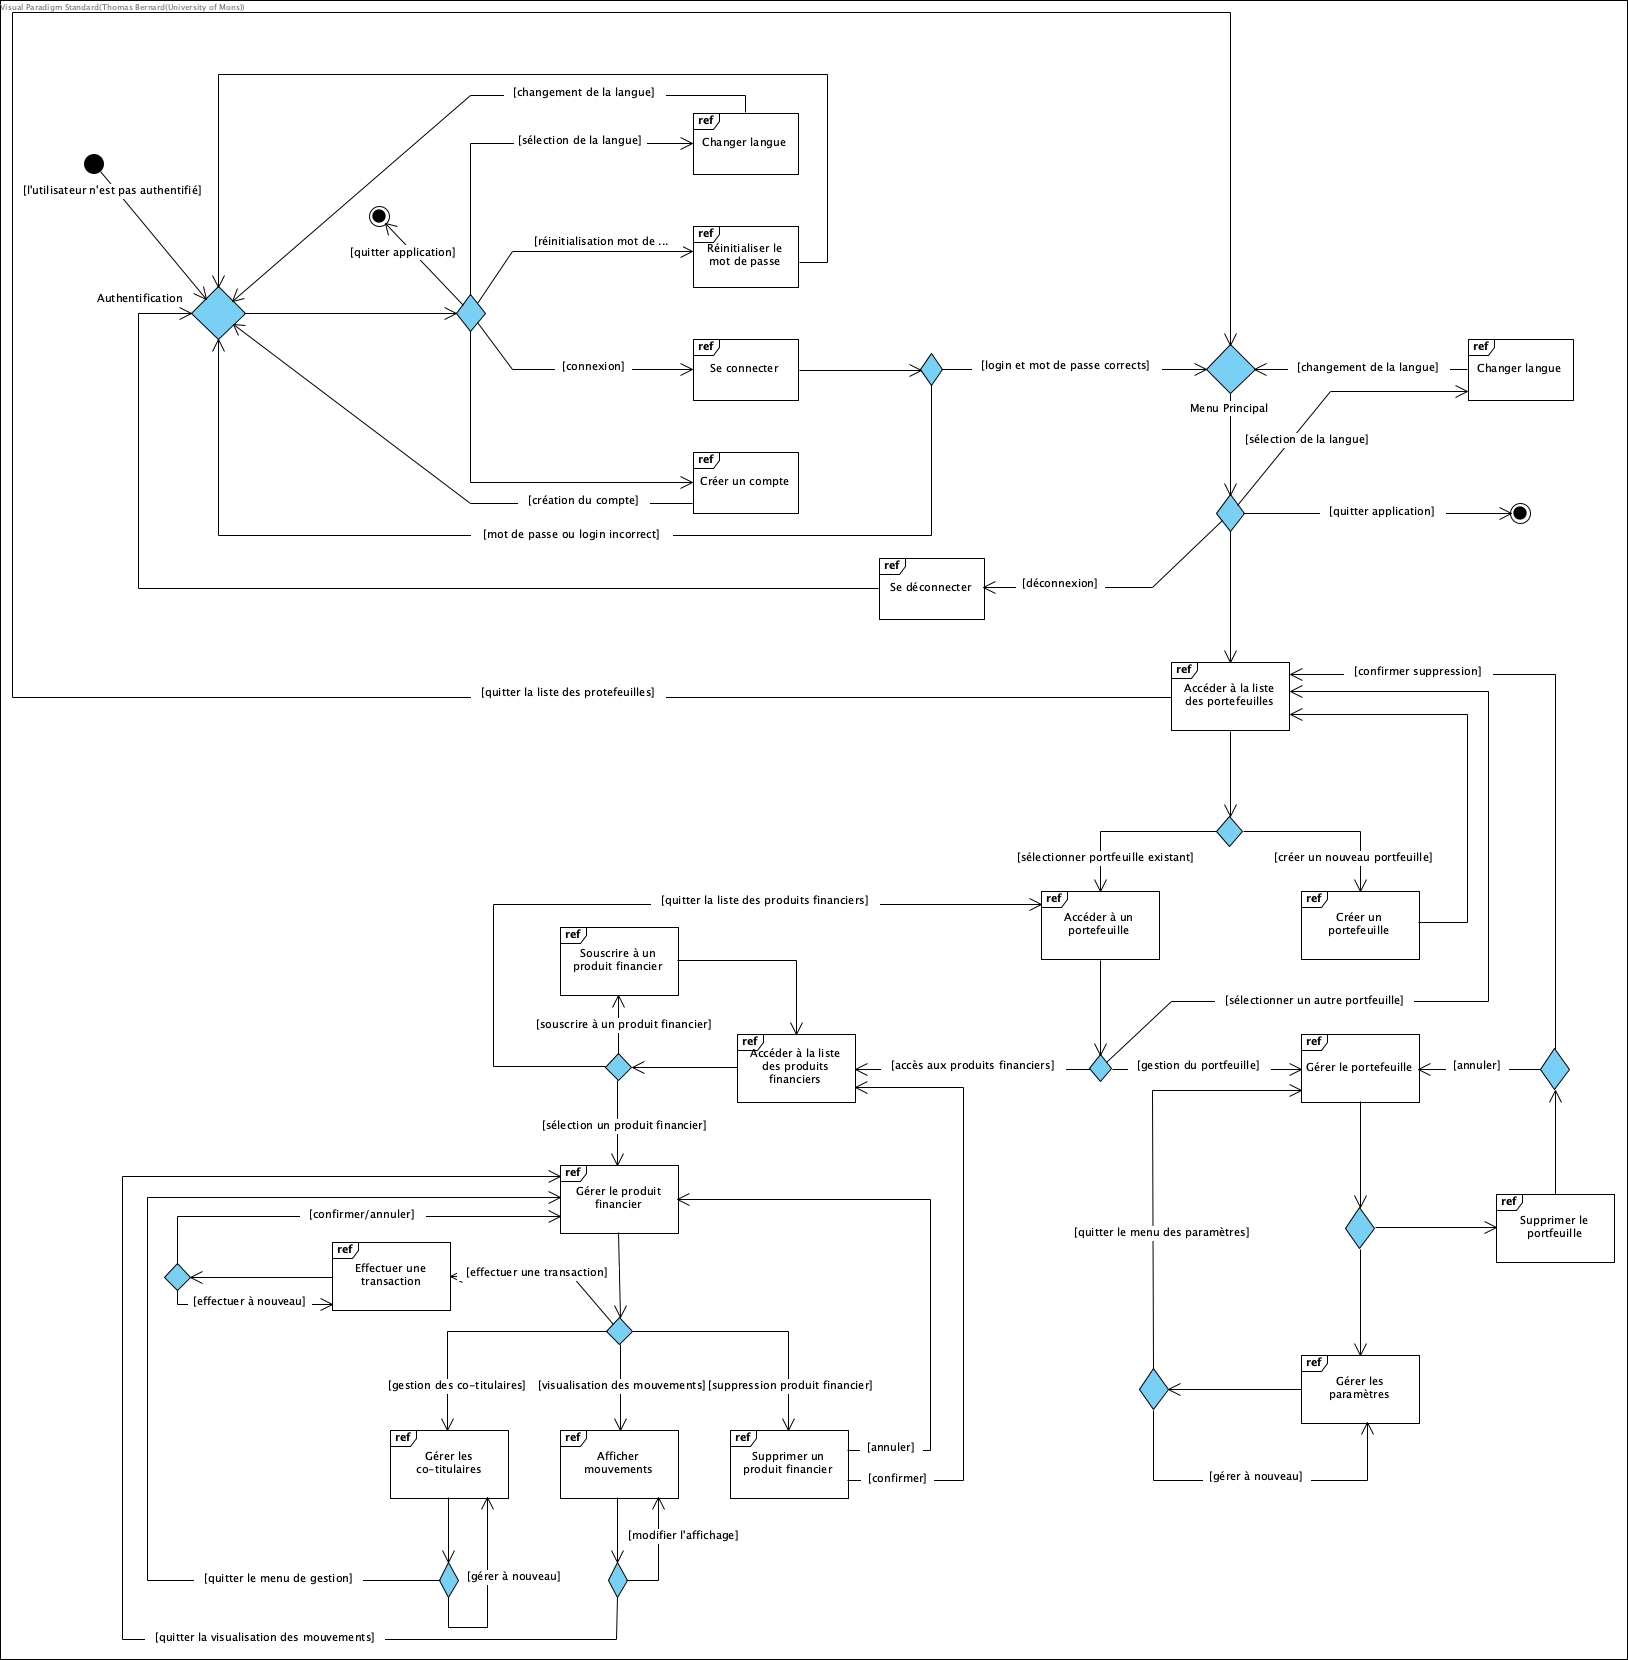
\includegraphics[scale=0.20]{ressources/photos_diagrammes/app1/int_over_app1.jpg}
		\caption{Interaction Overview Diagram Application 1.}
\end{figure}

Le schéma des intéractions de l'application utilisateurs est composée de 3 parties principales. Une partie dédiée à l'accès à l'application (authentification), une partie pour la l'accès et la gestion des portefeuilles financiers la dernière pour l'accès et la gestion des produits financiers.\\
\newpage
\end{document}
